\documentclass[12pt,letterpaper,oneside,reqno]{amsart}
\usepackage{amsfonts}
\usepackage{amsmath}
\usepackage{amssymb}
\usepackage{amsthm}
\usepackage{float}
\usepackage{mathrsfs}
\usepackage{colonequals}
\usepackage[font=small,labelfont=bf]{caption}
\usepackage[left=1in,right=1in,bottom=1in,top=1in]{geometry}
\usepackage[pdfpagelabels,hyperindex,colorlinks=true,linkcolor=blue,urlcolor=magenta,citecolor=green]{hyperref}
\usepackage{graphicx}
\linespread{1.7}
\emergencystretch=1em
\usepackage{array}
\usepackage{etoolbox}
\usepackage{derivative}
\apptocmd{\sloppy}{\hbadness 10000\relax}{}{}
\raggedbottom

\newcommand \coeffA [3][A] {{\mathbf{#1}} \sb{#2,#3}}
\newcommand \polynomialP [4][P]{{\mathbf{#1}}\sp{#2} \sb{#3}(#4)}
\newcommand \bernoulli [2][B] {{#1}\sb{#2}}

% free foot note
\let\svthefootnote\thefootnote
\newcommand\freefootnote[1]{%
    \let\thefootnote\relax%
    \footnotetext{#1}%
    \let\thefootnote\svthefootnote%
}


\newtheorem{theorem}{Theorem}[section]
\newtheorem{corollary}[theorem]{Corollary}
\newtheorem{lemma}[theorem]{Lemma}
\newtheorem{example}[theorem]{Example}
\newtheorem{conjecture}[theorem]{Conjecture}
\newtheorem{definition}[theorem]{Definition}

\numberwithin{equation}{section}

\title[A novel proof of power rule in Calculus]
{A novel proof of power rule in Calculus}
\author[Petro Kolosov]{Petro Kolosov}
\address{Software Developer, DevOps Engineer}
\email{kolosovp94@gmail.com}
\urladdr{https://kolosovpetro.github.io}
\keywords{Calculus, Derivatives, Power rule, Binomial theorem, Differentiation}
\subjclass[2010]{26A24}
\date{\today}
\hypersetup{
    pdftitle={A novel proof of power rule in Calculus},
    pdfsubject={Calculus, Derivatives, Power Rule, Binomial theorem, Differentiation, Mathematics, Mathematical Analysis},
    pdfauthor={Petro Kolosov},
    pdfkeywords={Calculus, Derivatives, Power rule, Binomial theorem, Differentiation}
}
\begin{document}
    \begin{abstract}
        The power rule for derivatives, typically proven through the limit definition of derivative in conjunction with the
Binomial theorem.
In this manuscript we present an alternative approach to proving the power rule,
by utilizing a certain polynomial identity, such that expresses the function's growth.

    \end{abstract}

    \maketitle

    \tableofcontents

    \freefootnote{Sources: \url{https://github.com/kolosovpetro/ANovelProofOfPowerRuleInCalculus}}


    \section{Introduction and main results} \label{sec:introduction}
    Your introduction here.
Include some references~\cite{bayour2017truly,benkhettou2016conformable,caputo2009time,martins2009calculus,
    GithubSource_2022, Sloane_theencyclopedia}.
Lorem Ipsum is simply dummy text of the printing and typesetting industry.
Lorem Ipsum has been the industry's standard dummy text ever since the 1500s, when an unknown printer took a galley
of type and scrambled it to make a type specimen book.
It has survived not only five centuries, but also the leap into electronic typesetting, remaining essentially unchanged.
It was popularised in the 1960s with the release of Letraset sheets containing Lorem Ipsum passages, and more
recently with desktop publishing software like Aldus PageMaker including versions of Lorem Ipsum.

Figure example
\begin{figure}[H]
    \centering
    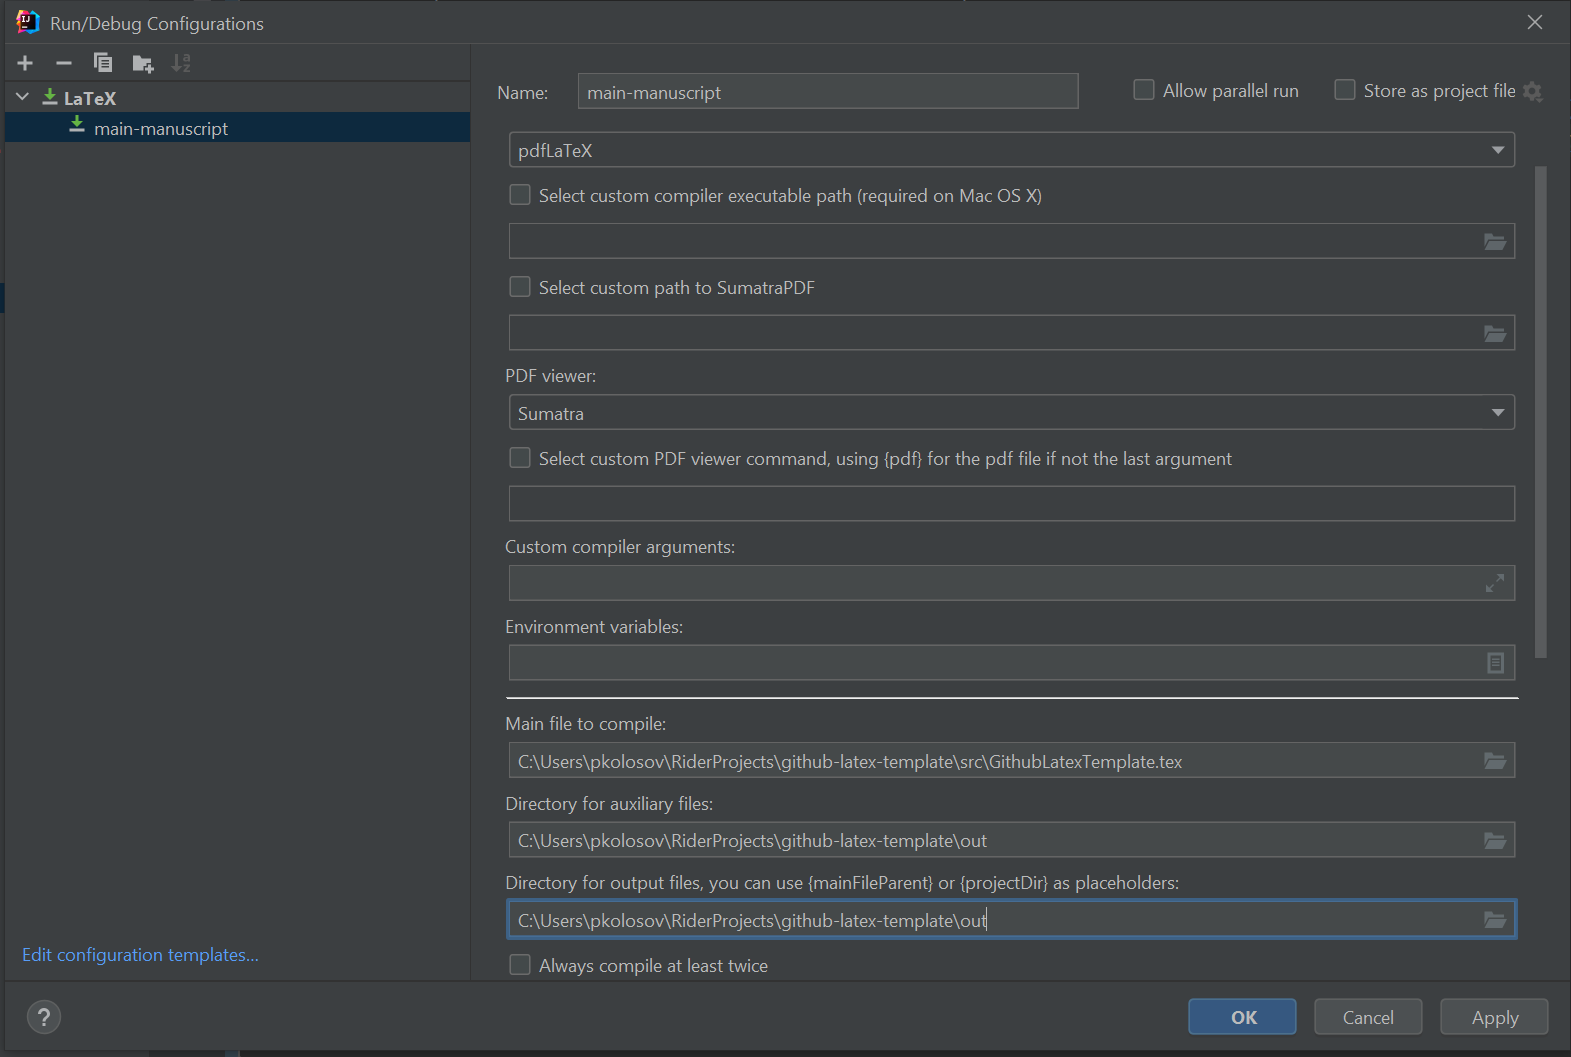
\includegraphics[width=1\textwidth]{../img/latex_configuration}
    ~\caption{Figure example.}\label{fig:figure}
\end{figure}

\begin{equation*}
     \llceil \nobarfrac{a}{b} \rrfloor_{m}
\end{equation*}
\begin{equation*}
    \llceilCoefficient{a}{b}{m}
\end{equation*}

And for any natural $m$ we have polynomial identity
\begin{equation}
    x^m = \sum_{k=1}^{m} T(m, k) \centralFactorial{x}{k}
    \label{eq:knuth-power-identity}
\end{equation}
where $\centralFactorial{x}{k}$ denotes central factorial defined by
\begin{equation*}
    \centralFactorial{x}{n} = x \fallingFactorial{x+\frac{n}{2}-1}{n-1}
\end{equation*}
where $\fallingFactorial{n}{k} = n (n-1) (n-2) \cdots (n-k+1)$ denotes falling factorial in Knuth's notation.
In particular,
\begin{equation*}
    \centralFactorial{x}{n}
    = x \left( x+\frac{n}{2}-1 \right) \left( x+\frac{n}{2}-1 \right) \cdots \left (x+\frac{n}{2}-n-1 \right)
    = x \prod_{k=1}^{n-1} \left( x+\frac{n}{2}-k \right)
\end{equation*}



%    \section{Conclusions}\label{sec:conclusions}
%    Conclusions of your manuscript.

    \bibliographystyle{unsrt}
    \bibliography{ANovelProofOfPowerRuleInCalculus}
    \noindent \textbf{Version:} \texttt{Local-0.1.0}


\end{document}
